\chapter{Radiative Corrections}
\label{cha:RadiativeCorrections}
%
When a cross-section is measured experimentally, the measurement yields the radiated cross-section plus contributions from radiated exclusive events, not the desired Born cross-section.
There are seven leading order contributions to the measured cross-section, summarized in figure~\ref{fig:radiatedFeynmanDiagrams}.
It is difficult, if not impossible, to distinguish these processes on the level of event selection, radiative corrections are therefore needed.
HAPRAD version 2.0 \cite{Akushevich99}\cite{Akushevich09} was used to calculate radiative corrections.
%
\begin{figure}[htp]
\centering
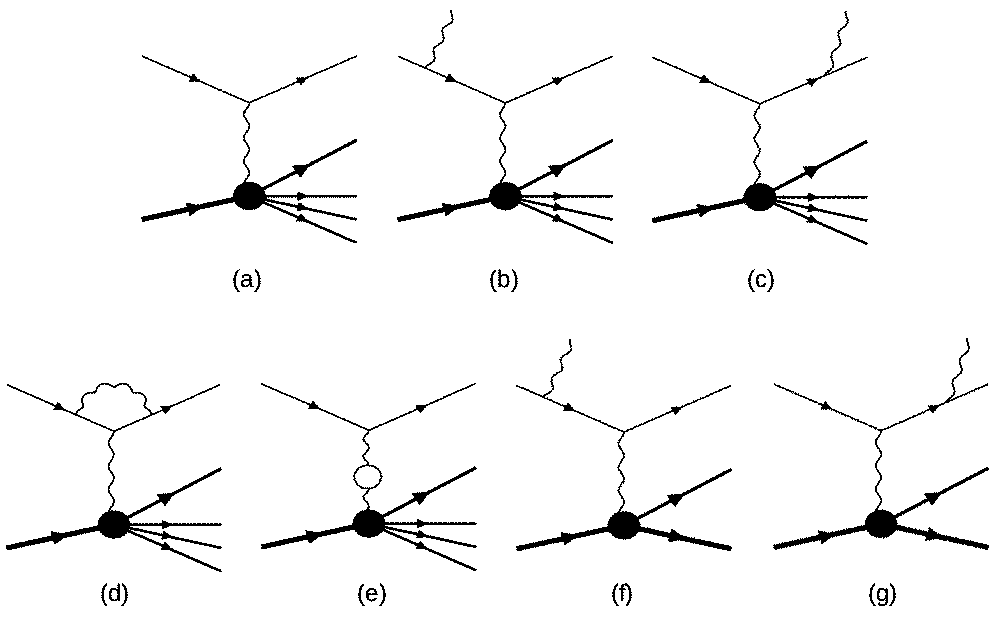
\includegraphics[width=5in]{figures/radiatedFeynmanDiagrams_BandW.png}
\caption{Feynman diagrams for contributions to the radiative cross-section. (a) The Born cross-section, (b) and (c) the emission of a radiated photon for SIDIS processes, (d) and (e) loop diagrams, and (f) and (g) emission of a radiated photon for exclusive processes.}
\label{fig:radiatedFeynmanDiagrams}
\end{figure}

HAPRAD works by calculating $\sigma_{rad+tail} \left( x, Q^2, z, P_{h\perp}^2, \phi_h \right)$ for a given \allowbreak $\sigma_{Born} \left( x, Q^2, z, P_{h\perp}^2, \phi_h \right)$ which is obtained from a model.
The radiative correction factor is then simply
\begin{equation}
\label{eq:RCfactor}
RC\ factor \left( x, Q^2, z, P_{h\perp}^2, \phi_h \right) = \frac{\sigma_{rad+tail} \left( x, Q^2, z, P_{h\perp}^2, \phi_h \right)}{\sigma_{Born} \left( x, Q^2, z, P_{h\perp}^2, \phi_h \right)}
\end{equation}
and the Born cross-section can be obtained by dividing the measured cross-section by the RC factor, i.e., $\sigma_{Born} = \sigma_{measured}/\text{RC factor}$.
Three different models were used to study model dependence, which proved to be a small effect (see chapter~\ref{cha:SystematicUncertainties} which discusses systematic uncertainties).
The three models used were (1) $A_{UU}^{\cos \phi_h} = A_{UU}^{\cos 2\phi_h} = 0$, (2) the ``default'' model that came with HAPRAD, which proved to describe the data reasonably well, and (3) an improved model based on the default model but with the parameters tuned to better match the data.
Model 3 was used for the final results and is shown for several bins in figures~\ref{fig:hapradModel_data_compare_pip} ($\pi^+$ channel) and~\ref{fig:hapradModel_data_compare_pim} ($\pi^-$ channel) along with the final results for comparison.
In the figures, the top row shows $A_{UU}^{\cos \phi_h}$ vs $P_{h\perp}^2$ and the bottom row shows $A_{UU}^{\cos 2\phi_h}$ vs $P_{h\perp}^2$; the columns are bins of $z$.
%
\begin{sidewaysfigure}[htp]
\centering
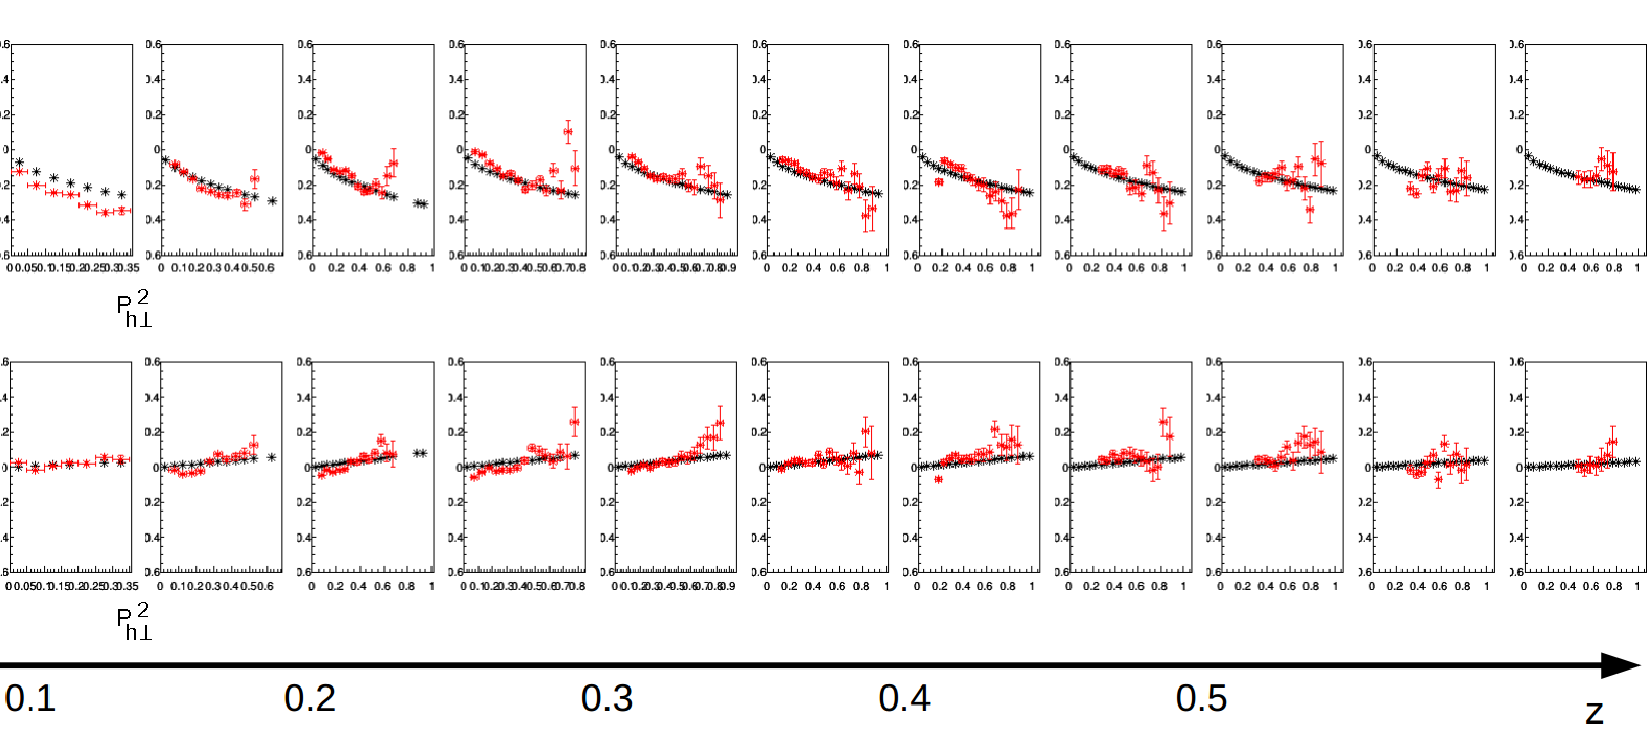
\includegraphics[width=8.5in]{figures/hapradModel_data_compare_pip.pdf}
\caption{The model for the Born cross-section used in HAPRAD (black points) and the experimental results (red points) for the $\pi^+$ channel. The top row shows $A_{UU}^{\cos \phi_h}$ vs $P_{h\perp}^2$ and the bottom row shows $A_{UU}^{\cos 2\phi_h}$ vs $P_{h\perp}^2$; the columns are bins of $z$. These results are for the high $Q^2$ of $ 0.1 < x < 0.2$.}
\label{fig:hapradModel_data_compare_pip}
\end{sidewaysfigure}
%
\begin{sidewaysfigure}[htp]
\centering
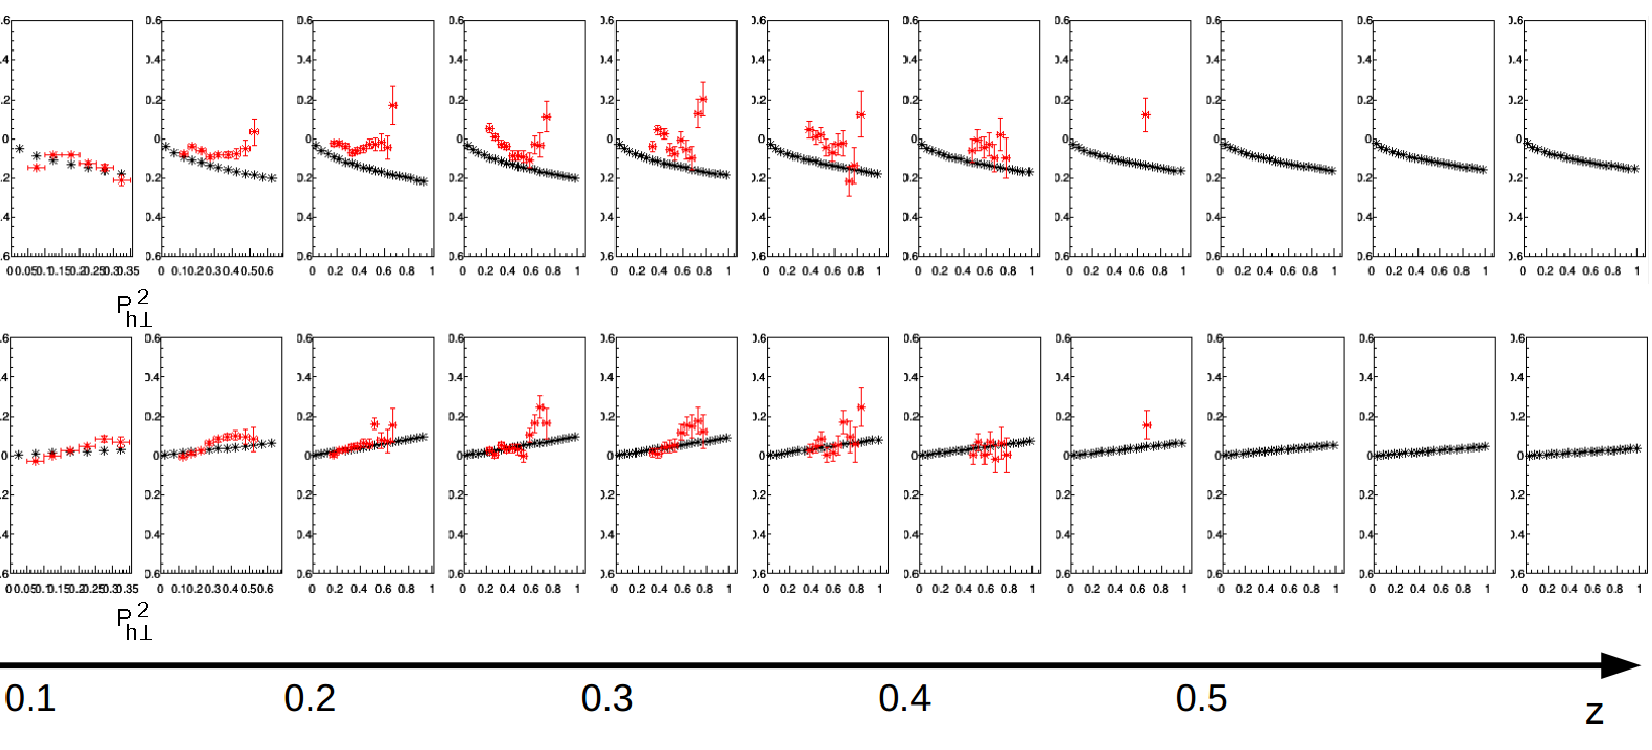
\includegraphics[width=8.5in]{figures/hapradModel_data_compare_pim.pdf}
\caption{The model for the Born cross-section used in HAPRAD (black points) and the experimental results (red points) for the $\pi^-$ channel. The top row shows $A_{UU}^{\cos \phi_h}$ vs $P_{h\perp}^2$ and the bottom row shows $A_{UU}^{\cos 2\phi_h}$ vs $P_{h\perp}^2$; the columns are bins of $z$. These results are for the high $Q^2$ of $ 0.1 < x < 0.2$.}
\label{fig:hapradModel_data_compare_pim}
\end{sidewaysfigure}
%

Some results from HAPRAD are shown in figures~\ref{fig:RCmagnitude_4D_intPhih} and~\ref{fig:RC_zPT2grid_x0QQ0}.
Figure~\ref{fig:RCmagnitude_4D_intPhih} shows the magnitude of the RC factor (integrated over $\phi_h$) as a function of $z$ and $P_{h\perp}^2$ for each of the nine $x$-$Q^2$ bins.
These results are very reasonable as they don't deviate very far from unity within the relevant kinematic ranges.
The kinematic region highlighted by the red rectangle in the bottom-left plot of figure~\ref{fig:RCmagnitude_4D_intPhih} is shown in more detail in figure~\ref{fig:RC_zPT2grid_x0QQ0}, which shows the $\phi_h$ dependence of $\sigma_{Born}$ (obtained from a model), $\sigma_{rad}$, and $\sigma_{tail}$ at different values of $z$ and $P_{h\perp}^2$ for fixed $x$ and $Q^2$.
%
\begin{sidewaysfigure}[htp]
\centering
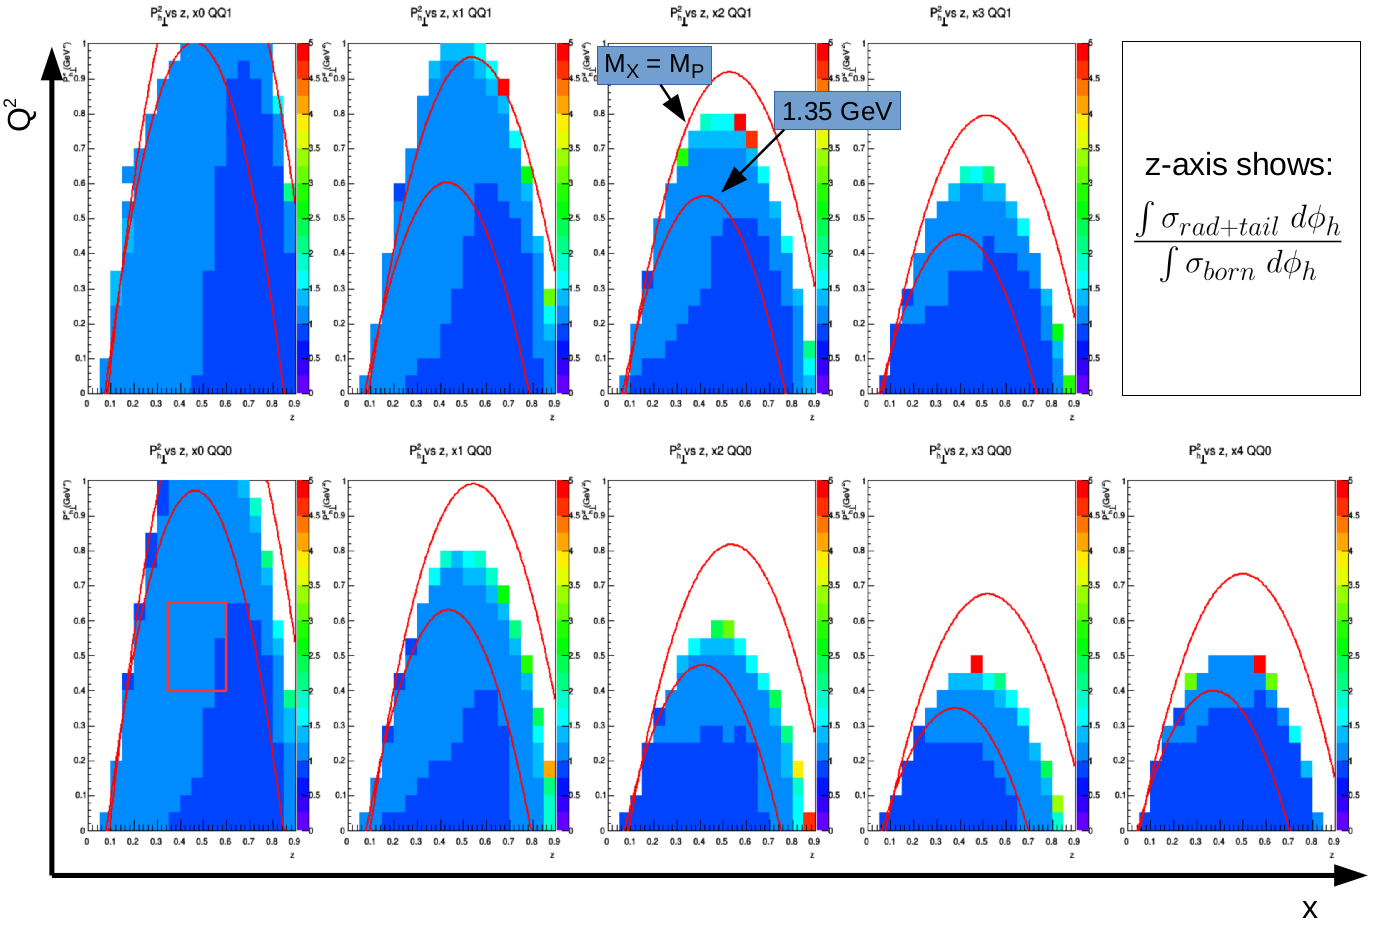
\includegraphics[width=8.5in]{figures/RCmagnitude_4D_intPhih.png}
\caption{$\int \sigma_{rad+tail} d\phi_h / \int \sigma_{Born} d\phi_h$ as a function of $z$ and $P_{h\perp}^2$ for each of the nine $x$-$Q^2$ bins.}
\label{fig:RCmagnitude_4D_intPhih}
\end{sidewaysfigure}
%
\begin{sidewaysfigure}[htp]
\centering
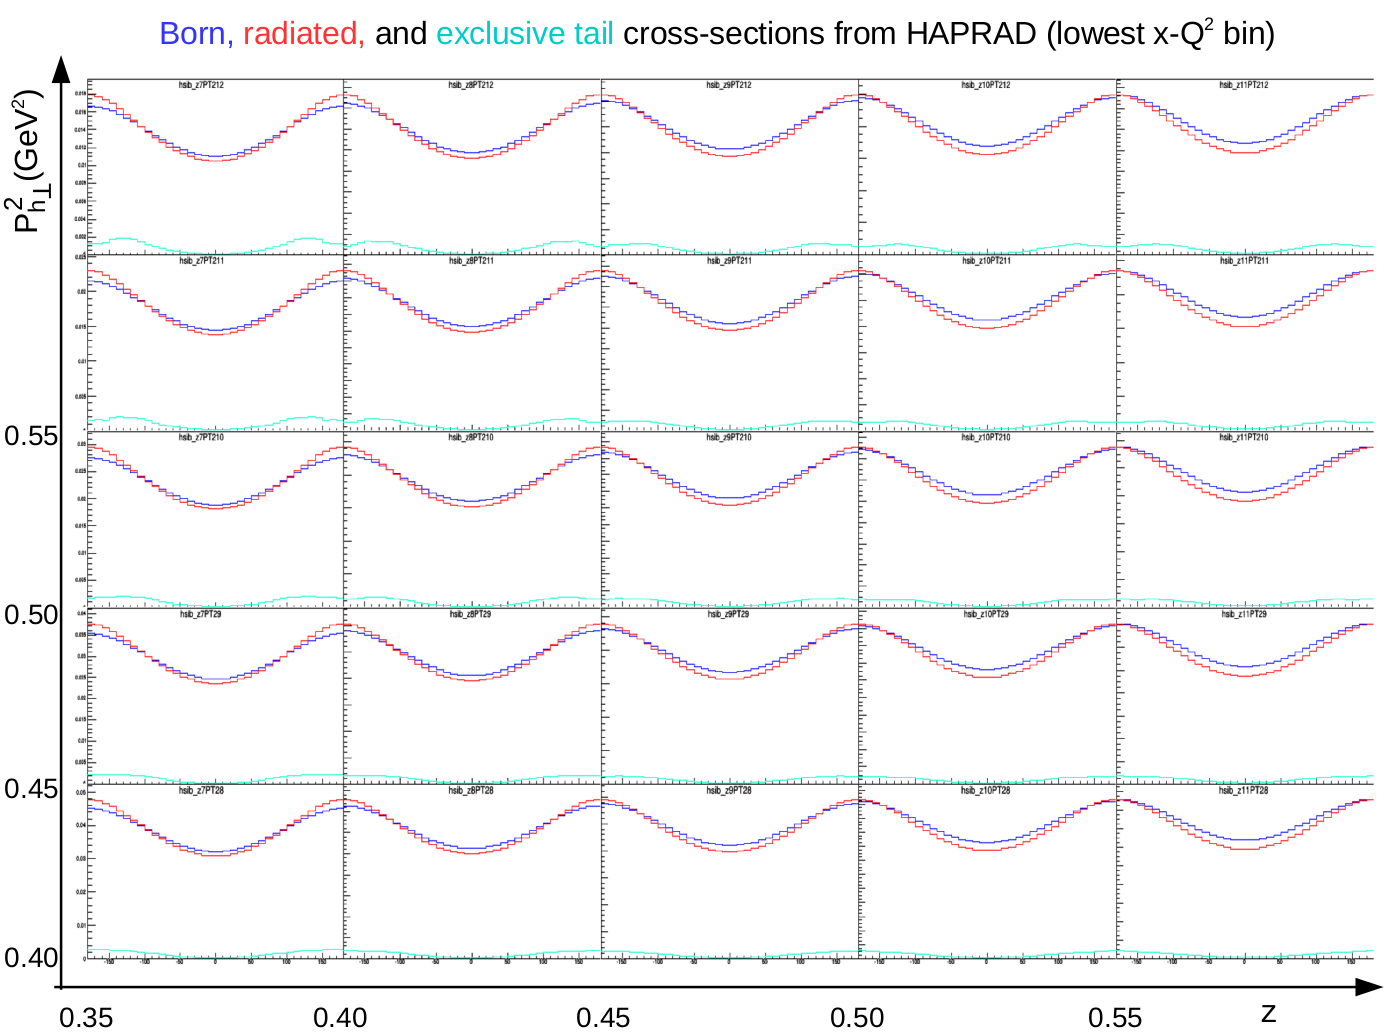
\includegraphics[width=8.5in]{figures/RC_zPT2grid_x0QQ0.png}
\caption{$\sigma_{Born}$ (blue), $\sigma_{rad}$ (red), and $\sigma_{tail}$ (teal) vs $phi_h$ for several points in $z$ and $P_{h\perp}^2$ and fixed $x$ and $Q^2$.}
\label{fig:RC_zPT2grid_x0QQ0}
\end{sidewaysfigure}
